\setlength{\doublerulesep}{0.3pt}

\themaN
\graphicspath{{../../S11_Multiples_et_diviseurs/Images/}}

\chapter{Multiples et\\diviseurs}
\label{S11}


%%%%%%%%%%%%%%%%%%%%%%%%%%%%%%%%
%%%%%%%%%%%%%%%%%%%%%%%%%%%%%%%%
\begin{autoeval}
   \small
   \begin{enumerate}
      \item Il calcule le quotient et le reste dans une division euclidienne.
      \item Il détermine si un nombre entier est ou n’est pas multiple ou diviseur d’un autre nombre entier.
      \item Il utilise les critères de divisibilité (par 2, 3, 5, 9, 10).
      \item Il modélise et résout des problèmes faisant intervenir les notions de multiple, de diviseur, de quotient et de reste.
   \end{enumerate}
\end{autoeval}

\begin{prerequis}[Connaissances $\heartsuit$ et compétences $\diamondsuit$ du cycle 4]
   \begin{itemize}
      \item Multiples et diviseurs.
      \item Critères de divisibilité par 2, 3, 5, 9.
      \item Division euclidienne.
      \item[\com] Déterminer si un entier est ou n'est pas multiple ou diviseur d'un autre entier.
      \item[\com] Utiliser un critère de divisibilité par 2, 3, 5, 9, 10.
      \item[\com] Modéliser et résoudre des problèmes mettant en jeu la divisibilité.
   \end{itemize}
\end{prerequis}

\vfill

\begin{debat}[Débat : la division euclidienne] 
   Le nom de {\bf division euclidienne} est un hommage rendu à {\it Euclide} (300 av. J.-C.), mathématicien grec qui en explique le principe par soustractions successives dans son \oe uvre {\it Les éléments}. Mais elle apparait très tôt dans l'histoire des mathématiques, par exemple dans les mathématiques égyptiennes, babyloniennes et chinoises.
   \begin{center}
      \begin{pspicture}(0,1.25)(4,4.25)
         \psline[linewidth=1mm](2,1)(2,4)
         \psline[linewidth=1mm](2,3)(4,3)
         \textcolor{B1}{\it\large
         \rput(0.8,3.5){dividende}
         \rput(3,3.5){diviseur}
         \rput(3,2.5){quotient}
         \rput(3,2){\small (euclidien)}
         \rput(1,1.5){reste}}
      \end{pspicture}
   \end{center}
   \bigskip
   \begin{cadre}[B2][J4]
      \begin{center}
         Vidéo : \href{https://www.youtube.com/watch?v=VWS9NyXbEyY&t=18s}{\bf Division euclidienne avec matériel multibase}, chaîne YouTube {\it Méthode Heuristique}.
      \end{center}
   \end{cadre}
\end{debat}


%%%%%%%%%%%%%%%%%%%%%%%%%%%%%%%
%%%%%%%%%%%%%%%%%%%%%%%%%%%%%%%
\activites

\begin{activite}[Les multiplications incomplètes]
   {\bf Objectifs} : calculer mentalement des multiplications et des divisions ; résoudre un problème de calcul mental ; compléter un tableau à double entrée.
   \begin{QCM}
   Compléter ces tables de multiplication dont on a effacé le contenu de certaines cases. Les nombres sont tous strictement positifs, il ne peut pas y avoir deux fois le même nombre sur une même colonne ou une même ligne. \medskip
   {\hautab{1.82}
   \partie[piste verte] \medskip
      \hfill
      \begin{tabular}{|C{0.5}||C{0.5}|C{0.5}|}
         \hline
         {\Large $\times$} & & \\
         \hline\hline
         & & 24 \\
         \hline
         & 25 & 30 \\
         \hline
      \end{tabular}
      \hfill
      \begin{tabular}{|C{0.5}||C{0.5}|C{0.5}|}
         \hline
         {\Large $\times$} & & 7 \\
         \hline\hline
         & & 21 \\
         \hline
         4 & 8 & \\
         \hline
      \end{tabular}
      \hfill
      \begin{tabular}{|C{0.5}||C{0.5}|C{0.5}|}
         \hline
         {\Large $\times$} & 6 & \\
         \hline\hline
         & 24 & 32 \\
         \hline
         & 36 & \\
         \hline
      \end{tabular}
      \hfill
      \begin{tabular}{|C{0.5}||C{0.5}|C{0.5}|}
         \hline
         {\Large $\times$} & 3 & \\
         \hline\hline
         & & 18 \\
         \hline
         5 & & 45 \\
         \hline
      \end{tabular}
      \hspace*{1cm} \\
         
   \partie[piste bleue] \medskip
      \hfill
      \begin{tabular}{|C{0.5}||C{0.5}|C{0.5}|C{0.5}|}
         \hline
         {\Large $\times$} & 2 & & \\
         \hline\hline
         & & 9 & \\
         \hline
         & 8 & & \\
         \hline
         & 16 & & 56 \\
         \hline
      \end{tabular}
      \hfill
      \begin{tabular}{|C{0.5}||C{0.5}|C{0.5}|C{0.5}|}
         \hline
         {\Large $\times$} & 2 & & \\
         \hline\hline
         4 & & 16 & \\
          \hline
         & & & 35 \\
         \hline
         9 & 18 & & 45 \\
         \hline
      \end{tabular}
      \hfill
      \begin{tabular}{|C{0.5}||C{0.5}|C{0.5}|C{0.5}|}
         \hline
         {\Large $\times$} & & 7 & \\
         \hline\hline
         & 12 & & 32 \\
         \hline
         & & & 64 \\
         \hline
         & & 63 & 72 \\
         \hline
      \end{tabular}
      \hspace*{1cm} \\
      
   \partie[piste rouge] \medskip 
      \hfill
      \begin{tabular}{|C{0.5}||C{0.5}|C{0.5}|C{0.5}|}
         \hline
         {\Large $\times$} & & 3 & \\
         \hline\hline
         & 20 & & \\
         \hline
         & & 18 & \\
         \hline
         & & 6 & 4 \\
         \hline
      \end{tabular}
      \hfill
      \begin{tabular}{|C{0.5}||C{0.5}|C{0.5}|C{0.5}|}
         \hline
         {\Large $\times$} & & & 7 \\
         \hline\hline
         2 & & & 14 \\
         \hline
         & 72 & 54 & \\
          \hline
         & 40 & & 35 \\
         \hline
      \end{tabular}
      \hfill
      \begin{tabular}{|C{0.5}||C{0.5}|C{0.5}|C{0.5}|}
         \hline
         {\Large $\times$} & & & \\
         \hline\hline
         & 18 & & 15 \\
         \hline
         & & 64 & \\
         \hline
         & & 32 & \\
         \hline
      \end{tabular}
      \hspace*{1cm} \\
      
   \partie[piste noire] \medskip
      \hfill
      \begin{tabular}{|C{0.5}||C{0.5}|C{0.5}|C{0.5}|}
         \hline
         {\Large $\times$} & & & 10 \\
         \hline\hline
         & 20 & 8 & \\
         \hline
         & 35 & & 70 \\
         \hline
         & & & 100 \\
         \hline
      \end{tabular}
      \hfill
      \begin{tabular}{|C{0.5}||C{0.5}|C{0.5}|C{0.5}|}
         \hline
         {\Large $\times$} & & & \\
         \hline\hline
         & & 45 & \\
         \hline
         & 28 & & \\
         \hline
         & 44 & & 99 \\
         \hline
      \end{tabular}
      \hfill
      \begin{tabular}{|C{0.5}||C{0.5}|C{0.5}|C{0.5}|}
         \hline
         {\Large $\times$} & & 13 & \\
         \hline\hline
         & & 65 & \\
         \hline
         & 42 & & 49 \\
         \hline
         & 72 & & 84 \\
         \hline
      \end{tabular}}
      \hspace*{1cm}
      \vspace*{1cm}
   \end{QCM}
\end{activite}


%%%%%%%%%%%%%%%%%%%%%%%%%%%%%%%
%%%%%%%%%%%%%%%%%%%%%%%%%%%%%%%
\cours 

%%%%%%%%%%%%%%%
\section{Multiples et diviseurs}

\begin{minipage}{10cm}
   {\it Rappel :} effectuer une division euclidienne d'un {\bf dividende} $a$ par un {\bf diviseur} $b$, c'est trouver deux entiers appelés {\bf quotient} $q$ et {\bf reste} $r$ tels que $a=b\times q+r$ où $r<b$. \\
   Dans l'exemple ci-contre, on peut écrire : $123 =5\times24+3$.
\end{minipage}
\qquad
\begin{minipage}{4cm}
   \begin{pspicture}(-0.5,-0.5)(4,3)
      \rput(1,1.2){$\opidiv[displayintermediary=all,voperation=top]{123}{5}$}
      \psline[linecolor=A1]{->}(0.7,2.8)(0.7,2.4)
      \rput(0.7,3){\textcolor{A1}{dividende}}
      \psline[linecolor=A1]{<-}(1.9,2.3)(2.4,2.3)
      \rput[l](2.5,2.3){\textcolor{A1}{diviseur}}
      \psline[linecolor=B1]{<-}(2.2,1.7)(2.7,1.7)
      \rput[l](2.8,1.7){\textcolor{B1}{quotient}}
      \psline[linecolor=B1]{<-}(1.4,0.2)(1.9,0.2)
      \rput[l](2,0.2){\textcolor{B1}{reste}}
   \end{pspicture}
\end{minipage}

\begin{definition}
   $a$ et $b$ sont deux nombres entiers. Lorsque le reste de la division de $a$ par $b$ est égal à 0, on dit que $a$ est un \textbf{multiple} de $b$, ou que $b$ est un \textbf{diviseur} de $a$, ou que $a$ est \textbf{divisible} par $b$.
\end{definition}

\begin{exemple*1}
   \begin{itemize}
      \item 15 est un multiple de 3 car $15=3\times 5+\textcolor{A1}{0}$, on peut aussi dire que 3 est un diviseur de 15, ou que 15 est divisible par 3.
      \item 17 n'est pas un multiple de 3 car $17=3\times 5+\textcolor{A1}{2}$.
      \item Les diviseurs de 24 sont 1; 2; 3; 4; 6; 8; 12 et 24.
      \item Il y a une infinité de multiples de 18, comme par exemple 18 ; 36 ; 54 ; 180\dots
   \end{itemize}
   \vspace*{-3mm}
\end{exemple*1}

%%%%%%%%%%%%%%%%%%%%%%%%%%
\section{Critères de divisibilité}

\begin{propriete}
   \begin{itemize}
      \item un nombre est divisible par 2 s'il se termine par 0 ; 2 ; 4 ; 6 ou 8 ;
      \item un nombre est divisible par 3 si la somme de ses chiffres est un multiple de 3 ;
      \item un nombre est divisible par 5 s'il se termine par 0 ou 5 ;
      \item un nombre est divisible par 9 si la somme de ses chiffres est un multiple de 9 ;
      \item un nombre est divisible par 10 s'il se termine par 0.
   \end{itemize}
   \vspace*{-3mm}
\end{propriete}

\begin{exemple*1}
   \begin{itemize}
      \item 252 et 253 sont-ils divisibles par 3 ?
      \item 52\,362 et 52\,363 sont-ils divisibles par 9 ?
    \end{itemize}   
   \correction
      \begin{itemize}
         \item $2+5+2=9$ est multiple de 3 donc, 252 est divisible par 3. \\
            $2+5+3=10$ n'est pas multiple de 3 donc, 253 n'est pas divisible par 3.
         \item $5+2+3+6+2=18$ est multiple de 9 donc, 52\,362 est divisible par 9, et donc par 3. \\
            $5+2+3+6+3=19$ n'est pas multiple de 9 donc, 52\,363 n'est pas divisible par 9.
       \end{itemize}
    \vspace*{-3mm}
\end{exemple*1}

\begin{remarque}
   pour savoir si un nombre est divisible par $3$, on peut calculer la somme des chiffres du nombre obtenu jusqu'à ce que l'on trouve un seul chiffre : \\
   pour $563\,387\,981$, on calcule : $5+6+3+3+8+7+9+8+1=50$. Puis on calcule $5+0=5$.
   $5$ n'est pas divisible par $3$ donc, $563\,387\,981$ n'est pas divisible par $3$.
\end{remarque}


%%%%%%%%%%%%%%%%%%%%%%%%%%%%%%%
%%%%%%%%%%%%%%%%%%%%%%%%%%%%%%%
\exercicesbase

\begin{colonne*exercice}

\begin{exercice} %1
   Effectuer les divisions euclidiennes suivantes :
   \begin{itemize}
      \item 307 par 7 ;
      \item 13\,758 par 25.
   \end{itemize}
\end{exercice}
        
\begin{corrige}
   {\small \opidiv[displayintermediary=all,voperation=top]{307}{7} \hfill \opidiv[displayintermediary=all,voperation=top]{13758}{25}} \\
   {\blue $307 =7\times43+6$} \hfill et \hfill {\blue $13\,758 =25\times550+8$}.
\end{corrige}

\bigskip


\begin{exercice} %2
   On donne les égalités : \\
   $415 = 7\times59+2$ \; et \; $56\times57 = 3\,192$. \\
   Sans effectuer de calculs, donner le quotient et le reste des divisions euclidiennes suivantes.
   \begin{colenumerate}{2}
      \item 415 par 7
      \item 3\,192 par 56
      \item 415 par 59
      \item 3\,192 par 57
   \end{colenumerate}
\end{exercice}

\begin{corrige}
   \ \\ [-5mm]
   \begin{enumerate}
      \item Le quotient de 415 par 7 est {\blue 59}, le reste est {\blue 2}.
      \item Le quotient de 3\,192 par 56 est {\blue 57}, le reste est {\blue 0}.
      \item Le quotient de 415 par 59 est {\blue 7}, le reste est {\blue 2}.
      \item Le quotient de 3\,192 par 57 est {\blue 56}, le reste est {\blue 0}.
   \end{enumerate}
\end{corrige}

\bigskip


\begin{exercice} %3
   Résoudre les problèmes suivants :
   \begin{enumerate}
      \item 6\,798 supporters d'un club de rugby doivent faire un déplacement en car pour soutenir leur équipe. Chaque car dispose de 55 places. \\
        Combien de cars faut-il réserver ?
      \item Des stylos sont conditionnés par boîte de 40. Ashiderdene a 2\,647 stylos. \\
         Combien lui en manque-t-il pour avoir des boîtes entièrement remplies ?
      \item Trois amis participent à une chasse au trésor et trouvent 1\,419 pièces en chocolat. \\
      Si le partage est équitable, combien de pièces en chocolat auront-ils chacun ? \\
      Otmane arrive et leur rappelle que c'est lui qui leur a prêté sa boussole. Il exige donc d'avoir la même part que chacun des trois autres plus les pièces restantes. \\
      Combien de pièces recevra-t-il ?
   \end{enumerate}
\end{exercice}

\begin{corrige}
   \ \\ [-5mm]
   \begin{enumerate}
      \item On effectue la division : {\small \opidiv[displayintermediary=all,voperation=top]{6798}{55}} \\
         En prenant 123 cars, il restera 33 personnes, il faudra donc réserver {\blue 124 cars}.
      \item On effectue la division : {\small \opidiv[displayintermediary=all,voperation=top]{2647}{40}} \\
         Il lui reste 7 stylos pour une boite de 40, il faut donc ajouter {\blue 33 stylos} pour compléter la boite.
      \item On effectue la division : {\small \opidiv[displayintermediary=all,voperation=top]{1419}{3}} \\
         Chaque ami aura donc {\blue 473 pièces en chocolat} et il n'en restera	pas.
   \end{enumerate}
   
\Coupe


   Lorsque Otmane arrive, on fait {\small \opidiv[displayintermediary=all,voperation=top]{1419}{4}} \\
   Il recevra $(354+3)$ pièces en chocolat, soit {\blue 357}. \\
\end{corrige}

\bigskip


 \begin{exercice} %4
   Trouver tous les diviseurs des nombres suivants :
   \begin{colitemize}{2}
      \item 14
      \item 40
      \item 48
      \item 2\,037
   \end{colitemize}
\end{exercice}

\begin{corrige}
   \begin{itemize}
      \item Diviseurs de 14 : {\blue 1 ; 2 ; 7 ; 14}.
      \item Diviseurs de 40 : {\blue 1 ; 2 ; 4 ; 5 ; 8 ; 10 ; 20 ; 40}.
      \item Diviseurs de 48 : {\blue 1 ; 2 ; 3 ; 4 ; 6 ; 8 ; 12 ; 16 ; 24 ; 48}.
      \item Diviseurs de 2\,037 : {\blue 1 ; 3 ; 7 ; 21 ; 97 ; 291 ; 679 ; 2037}.
   \end{itemize}
\end{corrige}

\bigskip


\begin{exercice} %5
   Ecrire :
   \begin{enumerate}
      \item La liste des dix premiers multiples de 6.
      \item Cinq multiples de 11.
      \item Tous les multiples de 13 inférieurs à 80.
      \item Le plus grand multiple de 12 inférieur à 75.
      \item Le plus grand multiple de 36 inférieur à 100.
      \item Le plus petit multiple de 9 supérieur à 1\,200.
      \item Le plus petit multiple de 14 supérieur à 710 ?
      \item Le plus petit et le plus grand diviseur de 2\,021.
   \end{enumerate}
\end{exercice}

\begin{corrige}
   \ \\ [-5mm]\begin{enumerate}
      \item Dix premiers multiples de 6 : \\
         {\blue 0 ; 6 ; 12 ; 18 ; 24 ; 30 ; 36 ; 42 ; 48 ; 54}.
      \item Cinq multiples de 11 : \\
         {\blue 0 ; 11 ; 22 ; 33 ; 44}.
      \item Multiples de 13 inférieurs à 80 : \\
         {\blue 0 ; 13 ; 26 ; 39 ; 52 ; 65 ; 78}
      \item Plus grand multiple de 12 inférieur à 75 : {\blue 72}.
      \item Plus grand multiple de 36 inférieur à 100 : {\blue 72}.
      \item Plus petit multiple de 9 supérieur à 1\,200 : {\blue 1206}.
      \item Plus petit multiple de 14 supérieur à 710 : {\blue 714}.
      \item Plus grand/petit diviseur de 2\,021 : {\blue 1 et 2\,021}.
   \end{enumerate}
\end{corrige}

\bigskip


\begin{exercice} %6
   Je suis un nombre impair à deux chiffres sans 2 dans mon écriture. Je ne suis pas divisible par 5 mais je suis un multiple de 9. \\
   Qui suis-je ? 
\end{exercice}

\begin{corrige}
   \begin{itemize}
      \item On peut commencer par écrire la liste des multiples de 9 à deux chiffres : \\
         18 ; 27 ; 36 ; 45 ; 54 ; 63 ; 72 ; 81 ; 90 ; 99.
      \item On supprime ensuite les nombres pairs, il reste : \\
         27 ; 45 ; 63 ; 81 ; 99.
      \item On supprime 27 qui comporte un 2, il reste : \\
         45 ; 63 ; 81 ; 99. \\
      \item Enfin, on supprime 45 qui est divisible par 5. \\
         Je peux donc être {\blue 63, 81 ou 99}.
   \end{itemize}
\end{corrige}

\bigskip


\begin{exercice} %7
   Les nombres 30 ; 27 ; 246 ; 325 ; 4\,238 et 6\,139 sont-ils divisibles par 2 ? par 3 ? par 5 ? par 9 ?
\end{exercice}

\begin{corrige}
   On résume les résultats dans un tableau : \\ \medskip
   {\hautab{1}
   \begin{CLtableau}{0.95\linewidth}{7}{c}
      \hline
      & 30 & 27 & 246 & 325 & \!4\,238 & \!6\,139 \\
      \hline
      par 2 & \textcolor{blue}{$\times$} & & \textcolor{blue}{$\times$} & & \textcolor{blue}{$\times$} & \\
      \hline
      par 3 & \textcolor{blue}{$\times$} & \textcolor{blue}{$\times$} & \textcolor{blue}{$\times$} & & & \\
      \hline
      par 5 & \textcolor{blue}{$\times$} & & & \textcolor{blue}{$\times$} & & \\
      \hline
      par 9 & & \textcolor{blue}{$\times$} & & & & \\
      \hline
   \end{CLtableau}}
\end{corrige}

\bigskip


\begin{exercice} %8
   Relier les deux cases colorées en suivant un chemin constitué uniquement de multiples de 6. \\ [1mm]
   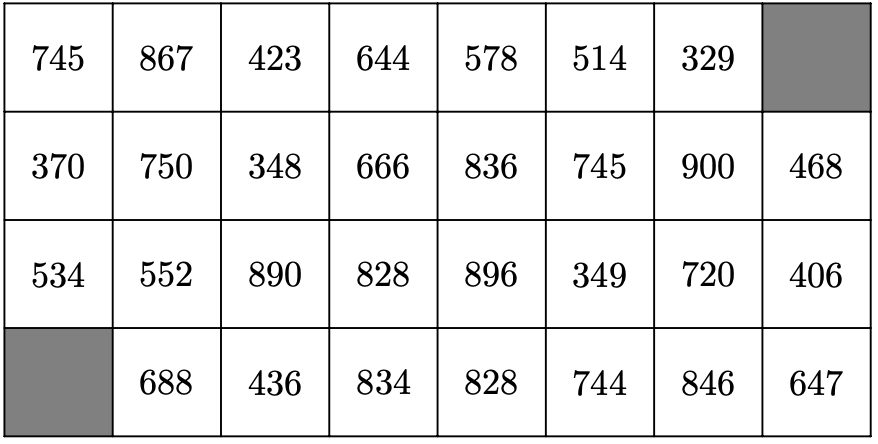
\includegraphics[width=8.2cm]{labynombre6}
\end{exercice}

\begin{corrige}
   \ \\ [-3mm]
   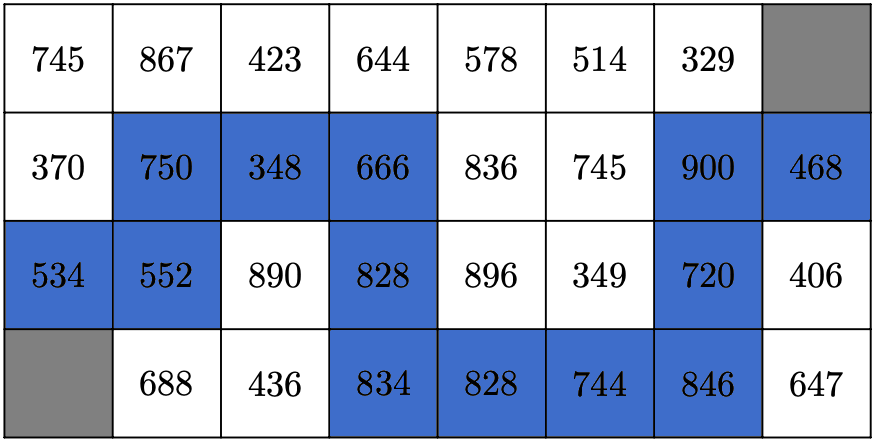
\includegraphics[width=7.5cm]{../../S11_Multiples_et_diviseurs/Images/labynombre6_corr}
   %\LabyNombre[Multiple=6,Couleur=Gray,Longueur=8,YDepart=0,YArrivee=3,Solution]
\end{corrige}

\smallskip


\begin{exercice} %9
   Relier les deux cases colorées en suivant un chemin constitué uniquement de diviseurs de 9. \\ [1mm]
   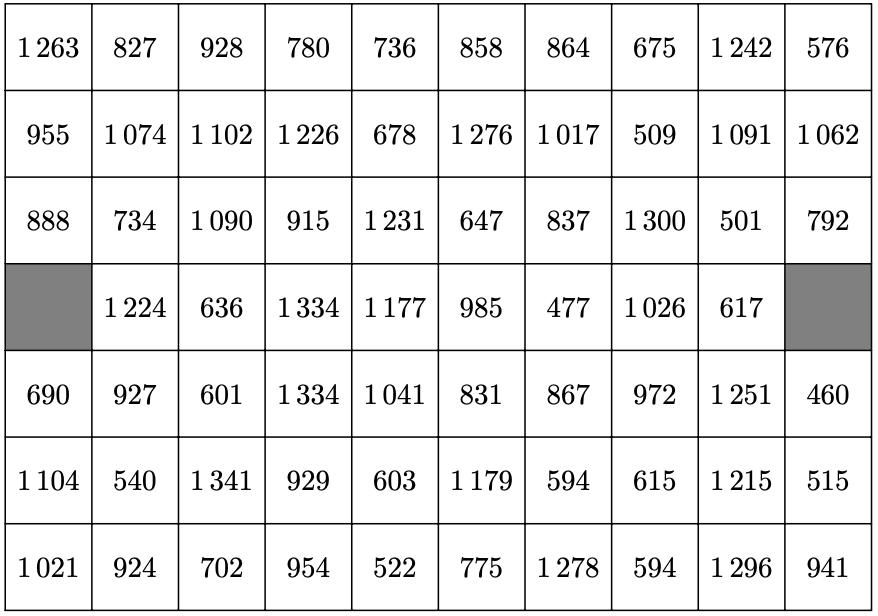
\includegraphics[width=8.2cm]{labynombre9}
\end{exercice}

\begin{corrige}
   \ \\ [-3mm]
   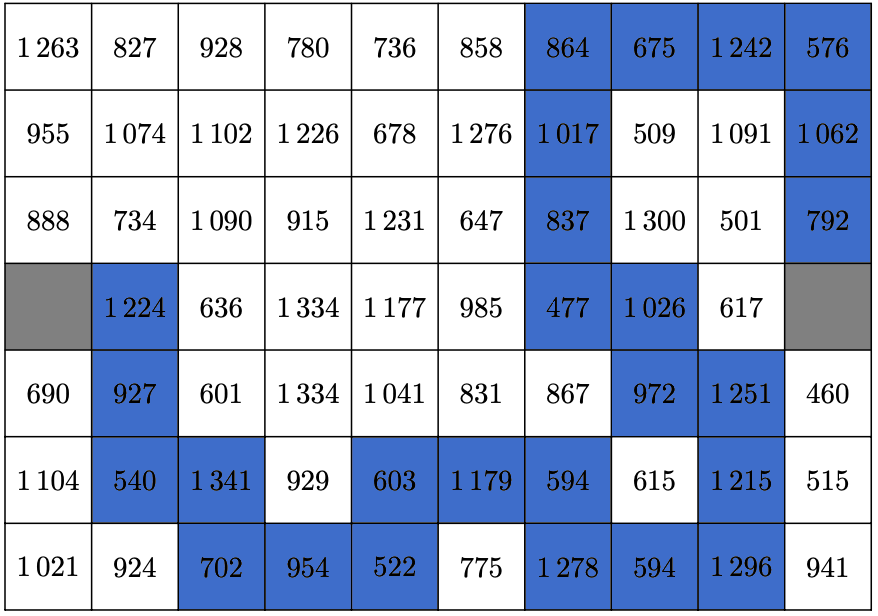
\includegraphics[width=7.5cm]{../../S11_Multiples_et_diviseurs/Images/labynombre9_corr}
   %\LabyNombre[Multiple=9,Couleur=Gray,Echelle=0.8,Longueur=10,Largeur=8,YDepart=3,XArrivee=9,YArrivee=3,Solution]
\end{corrige}

\smallskip


\begin{exercice} %10
   Répondre par vrai ou faux en justifiant.
   \begin{enumerate}
      \item Tout nombre divisible par 3 est divisible par 9.
      \item Tout nombre divisible par 9 est divisible par 3.
      \item Tout nombre divisible par 2 et 3 est divisible par 5.
      \item Tout nombre dont le chiffre des unités est 2 est divisible par 2. 
      \item Tout nombre dont le chiffre des unités est 3 est divisible par 3.
   \end{enumerate}
\end{exercice}

\begin{corrige}
   \ \\ [-5mm]
   \begin{enumerate}
      \item Tout nombre divisible par 3 est divisible par 9 : \\
         {\blue faux}. \\
         Par exemple, 6 est divisible par 3 mais pas par 9.
      \item Tout nombre divisible par 9 est divisible par 3 : \\
         {\blue vrai}. \\
         Un nombre divisible par 9 s'écrit $9k$ où $k$ est un nombre entier. Or, $9k =3\times(3k)$ donc il est aussi divisible par 3.
      \item Tout nombre divisible par 2 et 3 est divisible par 5 : {\blue faux}. \\
      Par exemple, 6 est divisible par 2 et par 3 mais il n'est pas divisible par 5.
      \item Tout nombre dont le chiffre des unités est 2 est divisible par 2 : {\blue vrai}. \\
      Un nombre qui se termine par 0, 2, 4, 6 ou 8 est divisible par 2.
      \item Tout nombre dont le chiffre des unités est 3 est divisible par 3 : {\blue faux}. \\
      Par exemple, 13 se termine par 3 mais n'est pas divisible par 3.
   \end{enumerate}
\end{corrige}

\end{colonne*exercice}


%%%%%%%%%%%%%%%%%%%%%%%%%
%%%%%%%%%%%%%%%%%%%%%%%%%
\Recreation

\begin{enigme}[Shikaku]
   Le {\bf Shikaku} est un casse-tête japonais. Son nom vient du Japonais et signifie \og diviser en carrés \fg. \\
   Le but de ce jeu est de diviser une grille donnée en plusieurs rectangles. \medskip
      
   \partie[règle du jeu]
      \ \\[-11mm]
      \begin{itemize}
         \item Paver la grille à l'aide de rectangles.
         \item Chaque rectangle doit contenir un nombre et un seul.
         \item Le nombre contenu dans un rectangle indique combien de cases le constituent. \medskip
      \end{itemize}

   \partie[exemple]
      {\psset{unit=0.6,subgriddiv=0,gridlabels=0,gridwidth=0.15mm}\footnotesize
         \begin{tabular}{*{6}{C{2.5}}}
            \begin{pspicture}(0,0)(4,4)
               \psgrid(0,0)(4,4)
               \rput(3.5,3.5){4}
               \rput(2.5,2.5){6} \rput(3.5,2.5){3} 
               \rput(0.5,0.5){2} \rput(2.5,0.5){1}           
            \end{pspicture}
            &
            \begin{pspicture}(0,0)(4,4)
               \psgrid(0,0)(4,4)
               \rput(3.5,3.5){4}
               \rput(2.5,2.5){6} \rput(3.5,2.5){3} 
               \rput(0.5,0.5){2} \rput(2.5,0.5){1} 
              \psset{linewidth=0.6mm,linecolor=PartieStatistique}
               \psframe(2,0)(3,1)
            \end{pspicture}
            &
            \begin{pspicture}(0,0)(4,4)
               \psgrid(0,0)(4,4)
               \rput(3.5,3.5){4}
               \rput(2.5,2.5){6} \rput(3.5,2.5){3} 
               \rput(0.5,0.5){2} \rput(2.5,0.5){1} 
               \psset{linewidth=0.6mm,linecolor=PartieStatistique}
               \psframe(2,0)(3,1)
               \psframe(0,3)(4,4)
            \end{pspicture}
            &
            \begin{pspicture}(0,0)(4,4)
               \psgrid(0,0)(4,4)
               \rput(3.5,3.5){4}
               \rput(2.5,2.5){6} \rput(3.5,2.5){3} 
               \rput(0.5,0.5){2} \rput(2.5,0.5){1} 
               \psset{linewidth=0.6mm,linecolor=PartieStatistique}
               \psframe(2,0)(3,1)
               \psframe(0,3)(4,4)
               \psframe(3,0)(4,3)
            \end{pspicture}
            &
            \begin{pspicture}(0,0)(4,4)
               \psgrid(0,0)(4,4)
               \rput(3.5,3.5){4}
               \rput(2.5,2.5){6} \rput(3.5,2.5){3} 
               \rput(0.5,0.5){2} \rput(2.5,0.5){1} 
               \psset{linewidth=0.6mm,linecolor=PartieStatistique}
               \psframe(2,0)(3,1)
               \psframe(0,3)(4,4)
               \psframe(3,0)(4,3)
               \psframe(0,1)(3,3)
            \end{pspicture}
            &
            \begin{pspicture}(0,0)(4,4)
               \psgrid(0,0)(4,4)
               \rput(3.5,3.5){4}
               \rput(2.5,2.5){6} \rput(3.5,2.5){3} 
               \rput(0.5,0.5){2} \rput(2.5,0.5){1} 
               \psset{linewidth=0.6mm,linecolor=PartieStatistique}
               \psframe(2,0)(3,1)
               \psframe(0,3)(4,4)
               \psframe(3,0)(4,3)
               \psframe(0,1)(3,3)
               \psframe(0,0)(2,1)
            \end{pspicture}
            \\
            grille d'origine
            &
            un rectangle à 1 case est forcément un carré de côté 1
            &
            un rectangle à 4 cases est un carré de côté 2 ou un rectangle de côtés 1 et 4
            &
            un rectangle à 3 cases est un rectangle de côtés 1 et 3
            &
            un rectangle à 6 cases est un rectangle de côtés 2 et 3 ou de côtés 1 et 6
            &
            un rectangle à 2 cases est un rectangle de côtés 1 et 2 \\
         \end{tabular}} \smallskip

   \partie[let's go !!!]
       {\psset{unit=0.75,subgriddiv=0,gridlabels=0,gridwidth=0.15mm}\footnotesize
            \begin{pspicture}(0,0)(4,4)
               \psgrid(0,0)(4,4)
               \rput(0.5,3.5){2} \rput(1.5,3.5){2} \rput(2.5,3.5){4}
               \rput(0.5,1.5){2} \rput(1.5,1.5){3}
               \rput(3.5,0.5){3}
            \end{pspicture}
            \hfill
            \begin{pspicture}(0,0)(5,5)
               \psgrid(0,0)(5,5)
               \rput(0.5,4.5){3} \rput(3.5,4.5){4}
               \rput(2.5,3.5){2}
               \rput(3.5,2.5){4}
               \rput(1.5,1.5){2} \rput(2.5,1.5){2} \rput(3.5,1.5){2}
               \rput(0.5,0.5){2} \rput(2.5,0.5){4}
            \end{pspicture}
            \hfill
            \begin{pspicture}(0,0)(6,6)
               \psgrid(0,0)(6,6)
               \rput(0.5,5.5){4} \rput(1.5,5.5){5} \rput(4.5,5.5){3}
               \rput(2.5,4.5){3}
               \rput(3.5,3.5){6}
               \rput(4.5,2.5){4}
               \rput(3.5,1.5){2} \rput(4.5,1.5){2}
               \rput(0.5,0.5){2} \rput(2.5,0.5){5}
            \end{pspicture} \\ [5mm]
            \begin{pspicture}(-1,0)(7,7)
               \psgrid(0,0)(7,7)
               \rput(6.5,6.5){2}
               \rput(3.5,5.5){6} \rput(4.5,5.5){2} \rput(5.5,5.5){2} \rput(6.5,5.5){2}
               \rput(1.5,4.5){2} \rput(3.5,4.5){4}
               \rput(0.5,3.5){6} \rput(2.5,3.5){3}
               \rput(1.5,2.5){3} \rput(5.5,2.5){4}
               \rput(3.5,1.5){4} \rput(5.5,1.5){2} \rput(6.5,1.5){2}
               \rput(1.5,0.5){2} \rput(4.5,0.5){3}
            \end{pspicture}
            \hfill
            \begin{pspicture}(0,0)(10,9)
               \psgrid(0,0)(9,9)
               \rput(0.5,8.5){2}
               \rput(0.5,7.5){2} \rput(2.5,7.5){6} \rput(5.5,7.5){3} \rput(6.5,7.5){2} \rput(7.5,7.5){4}
               \rput(3.5,6.5){2} \rput(7.5,6.5){2}
               \rput(3.5,5.5){2} \rput(5.5,5.5){2}
               \rput(0.5,4.5){5} \rput(2.5,4.5){6} \rput(5.5,4.5){2} \rput(6.5,4.5){3} \rput(7.5,4.5){4}
               \rput(1.5,3.5){7} \rput(3.5,3.5){3}
               \rput(7.5,2.5){6}
               \rput(4.5,1.5){9}
               \rput(1.5,0.5){3} \rput(4.5,0.5){4} \rput(7.5,0.5){2}
            \end{pspicture}}
\end{enigme}

\begin{corrige}
   \begin{center}
   {\psset{unit=0.75,subgriddiv=0,gridlabels=0,gridwidth=0.15mm}
      \begin{pspicture}(0,0)(4,3.7) %1
         \psgrid(0,0)(4,4)
         \rput(0.5,3.5){2}
         \rput(1.5,3.5){2}
         \rput(2.5,3.5){4}
         \rput(0.5,1.5){2}
         \rput(1.5,1.5){3}
         \rput(3.5,0.5){3}
         {\psset{linewidth=0.4mm,linecolor=blue}
            \psframe(0,0)(1,2)
            \psframe(0,2)(1,4)
            \psframe(1,0)(4,1)
            \psframe(1,1)(4,2)
            \psframe(1,2)(2,4)
            \psframe(2,2)(4,4)}
      \end{pspicture}
      \hfill
      \begin{pspicture}(0,0)(5,4.7) %2
         \psgrid(0,0)(5,5)
         \rput(0.5,4.5){3} \rput(3.5,4.5){4}
         \rput(2.5,3.5){2}
         \rput(3.5,2.5){4}
         \rput(1.5,1.5){2} \rput(2.5,1.5){2} \rput(3.5,1.5){2}
         \rput(0.5,0.5){2} \rput(2.5,0.5){4}
         {\psset{linewidth=0.4mm,linecolor=blue}
            \psframe(0,0)(1,2)
            \psframe(0,2)(1,5)
            \psframe(1,0)(5,1)
            \psframe(1,1)(2,3)
            \psframe(1,3)(3,4)
            \psframe(1,4)(5,5)
            \psframe(2,1)(3,3)
            \psframe(3,1)(5,2)
            \psframe(3,2)(5,4)}
      \end{pspicture} \\ [7mm]
      \begin{pspicture}(0,0)(6,6) %3
            \psgrid(0,0)(6,6)
            \rput(0.5,5.5){4} \rput(1.5,5.5){5} \rput(4.5,5.5){3}
            \rput(2.5,4.5){3}
            \rput(3.5,3.5){6}
            \rput(4.5,2.5){4}
            \rput(3.5,1.5){2} \rput(4.5,1.5){2}
            \rput(0.5,0.5){2} \rput(2.5,0.5){5}
            {\psset{linewidth=0.4mm,linecolor=blue}
               \psframe(0,0)(1,2)
               \psframe(0,2)(1,6)
               \psframe(1,0)(6,1)
               \psframe(1,1)(2,6)
               \psframe(2,1)(4,2)
               \psframe(2,2)(6,3)
               \psframe(2,3)(3,6)
               \psframe(3,3)(6,5)
               \psframe(3,5)(6,6)
               \psframe(4,1)(6,2)}
         \end{pspicture} \\ [7mm]
         \vfill
         \begin{pspicture}(0,0)(7,7) %4
               \psgrid(0,0)(7,7)
               \rput(6.5,6.5){2}
               \rput(3.5,5.5){6} \rput(4.5,5.5){2} \rput(5.5,5.5){2} \rput(6.5,5.5){2}
               \rput(1.5,4.5){2} \rput(3.5,4.5){4}
               \rput(0.5,3.5){6} \rput(2.5,3.5){3}
               \rput(1.5,2.5){3} \rput(5.5,2.5){4}
               \rput(3.5,1.5){4} \rput(5.5,1.5){2} \rput(6.5,1.5){2}
               \rput(1.5,0.5){2} \rput(4.5,0.5){3}
               {\psset{linewidth=0.4mm,linecolor=blue}
                  \psframe(0,0)(2,1)
                  \psframe(0,1)(1,7)
                  \psframe(1,1)(2,4)
                  \psframe(1,4)(3,5)
                  \psframe(1,5)(4,7)
                  \psframe(2,0)(5,1)
                  \psframe(3,1)(5,3)
                  \psframe(3,3)(5,5)
                  \psframe(4,5)(5,7)
                  \psframe(5,0)(6,2)
                  \psframe(5,2)(7,4)
                  \psframe(5,4)(6,6)
                  \psframe(5,6)(7,7)
                  \psframe(6,0)(7,2)
                  \psframe(6,4)(7,6)}
            \end{pspicture} \\ [7mm]
            \vfill
            \begin{pspicture}(0,0)(9,9)
               \psgrid(0,0)(9,9)
               \rput(0.5,8.5){2}
               \rput(0.5,7.5){2} \rput(2.5,7.5){6} \rput(5.5,7.5){3} \rput(6.5,7.5){2} \rput(7.5,7.5){4}
               \rput(3.5,6.5){2} \rput(7.5,6.5){2}
               \rput(3.5,5.5){2} \rput(5.5,5.5){2}
               \rput(0.5,4.5){5} \rput(2.5,4.5){6} \rput(5.5,4.5){2} \rput(6.5,4.5){3} \rput(7.5,4.5){4}
               \rput(1.5,3.5){7} \rput(3.5,3.5){3}
               \rput(7.5,2.5){6}
               \rput(4.5,1.5){9}
               \rput(1.5,0.5){3} \rput(4.5,0.5){4} \rput(7.5,0.5){2}
               {\psset{linewidth=0.4mm,linecolor=blue}
                  \psframe(0,0)(3,1)
                  \psframe(0,1)(1,6)
                  \psframe(0,6)(1,8)
                  \psframe(0,8)(2,9)
                  \psframe(1,1)(2,8)
                  \psframe(2,1)(3,7)
                  \psframe(2,7)(5,9)
                  \psframe(3,0)(7,1)
                  \psframe(3,1)(4,4)
                  \psframe(3,4)(4,6)
                  \psframe(3,6)(5,7)
                  \psframe(4,1)(7,4)
                  \psframe(4,4)(6,5)
                  \psframe(4,5)(6,6)
                  \psframe(5,6)(6,9)
                  \psframe(6,4)(7,7)
                  \psframe(6,7)(7,9)
                  \psframe(7,0)(9,1)
                  \psframe(7,1)(9,4)
                  \psframe(7,4)(9,6)
                  \psframe(7,6)(9,7)
                  \psframe(7,7)(9,9)}
            \end{pspicture}}
   \end{center}
\end{corrige}

